\subsection{Loss functions}
The problem of decoy quality assessment is essentially a ranking
problem: we have to arrange decoys according to their similarity to
the corresponding native structure, as quantified by the GDT\_TS score
\cite{zemla2001casp4}, for instance. Such a ranking approach to the
problem of model quality assessment has recently been used by the
MQAPRank method \cite{jing2016sorting}, which, however, relies on a
support vector machine model and uses high-level features as
input.

%%% GL: We need a reference for the ``margin ranking loss''
%%% concept. Who used it first?
In the present work, we define the loss function in terms of the
margin ranking loss \ref{???} for each pair of decoys.
%%% GL: I'm simplifying the notation a bit, here. We don't really need
%%% the x_i notation, so I've replaced f(x_i) by f_i.
Let $\text{GDT\_TS}_i$ denote the global distance test total score of
decoy $i$ and let $y_{ij}$ be the ordering coefficient of two decoys
$i$ and $j$:
$$
y_{ij} = \begin{cases}
               1& \text{if }\text{GDT\_TS}_i \leq \text{GDT\_TS}_j \\
               -1& \text{if }\text{GDT\_TS}_i > \text{GDT\_TS}_j \\
            \end{cases}
$$
%
In this work we assume that $\text{GDT\_TS}\in [0,1]$.
%%% GL: Why do you write this? What is the actual range of GDT_TS?
%%% Don't leave the reader guessing...
%
Let $f_i$ denote the output of the network for decoy $i$. We use the
following expression for the pairwise ranking scoring function:
%%% GL: ``ranking scoring function'' or ``ranking loss function''?
%
$$
L_{ij} = w_{ij} \max \left[ 0, 1 - y_{ij} \cdot (f_i - f_j) \right]
$$
%
The term $w_{ij}$ represents the weight of each example and is defined
so that decoys with similar scores are removed from the training:
%
$$
w_{ij} = \begin{cases}
               1& \text{if } \left| \text{GDT\_TS}_i - \text{GDT\_TS}_j \right| > T \\
               0& \text{otherwise} \\ 
            \end{cases}
$$
%
where $T$ is a threshold constant set to 0.1 GDT\_TS unit.
%%% GL: What is a GDT_TS unit??? It's in Angstroms, right?

During the training procedure we load $N_\text{B} = 9$ decoy
structures of a given target into memory (a ``batch'') and compute the
output of the network and the average loss:
$$
L = \frac{1}{N_\text{B}^2} \sum_{i=1}^{N_\text{B}}\sum_{\substack{j=1\\j\neq i}}^{N_\text{B}} L_{ij}
$$
Afterwards, we compute the gradient of the average loss with respect
to the network parameters and update them using the Adam algorithm
\cite{kingma2014adam}.


\subsection{Evaluation criteria}
We evaluate the model using various correlation coefficients of the
scores and using the loss criterion. The latter is defined, for any
given protein, as the absolute difference between the GDT\_TS of the
best decoy and the GDT\_TS of the decoy with the lowest predicted
score $f$:
$$ 
\mathrm{Loss} = \left| \mathrm{max}_i(\text{GDT\_TS}_i) - \text{GDT\_TS}_{\mathrm{argmin}_i(f_i)} \right|
$$
%
The correlation coefficients between the $f$ score produced by the
model and the GDT\_TS score are computed for all decoys of a given
target in the test set, and are then averaged over all targets
(per-target average). Since the value of GDT\_TS increases with the
quality of a model but the value of $f$ decreases, an ideal QA
algorithm would show a correlation coefficient of $-1$ and a loss of
$0$.


\subsection{Optimization and dataset sampling}
The parameter optimization of the model was performed using the Adam
algorithm \cite{kingma2014adam}. The gradient of the loss function
with respect to the model parameters was computed on the pairs of
models in the batch. The batch size was set to $N_\text{B} = 9$
models.
%%% GL: We've introduced the notation N_B for the batch size earlier
%%% on. Moreover, variable M was used earlier for the number of
%%% filters.

%%% GL: Avoid ``we'' and ``our'' as much as possible. It sometimes
%%% sounds more lively but it usually give the results an air of
%%% subjectivity, as if somebody else would find different
%%% results. See what I did to the following paragraph:
The training dataset is sampled by first choosing a random target from
the dataset, then sampling decoys of this target. One epoch
corresponds to one pass through all targets in the dataset. The decoys
are sampled in a homogeneous way, by dividing all decoys of a given
target into $N_\text{B} = 9$ bins by the value of their GDT\_TS score
and picking one decoy from each bin at random.
%
Precisely, decoy $i$ belongs to the bin number $1 + \left[
  \max(\text{GDT\_TS}) - \text{GDT\_TS}_i \right] / \left[
  \max(\text{GDT\_TS}) - \min(\text{GDT\_TS}) \right]$, where
$\max(\text{GDT\_TS})$ and $\min(\text{GDT\_TS})$ are computed for all
decoys of the chosen target.
%%% GL: I repeat my comment: This isn't the formula for the bin
%%% number. Don't you need an integer from 1 to 9?
%
If a bin is empty, the decoy is picked from a non-empty bin chosen at
random (???), and so on until the batch is full. The order of targets
and the order of decoys are randomly shuffled at the end of each
epoch.
%%% GL: Do we need ``and so on until the batch is full''?

Decoy structures are randomly rotated and translated each time they
are used as input. The rotations are sampled uniformly
\cite{shoemake1992uniform} and the translation are chosen in such a
way that the translated protein fits inside the $120$~\AA${}\times
120$~\AA${}\times 120$~\AA\ input grid (see Supporting Information for
details).

We select the final model based on its performance on a
\emph{validation subset} consisting of 35 targets (and their decoys)
picked at random from the training set and excluded from the training
procedure. The remaining 529 targets are called the \emph{training
subset}.  Figure~\ref{Fig:TrainingLoss} shows the Kendall $\tau$ and
Pearson $R$ coefficients and the loss on the validation subset over 52
epochs of training.  Models are saved every 10 epochs and we pick the
one that has the smallest loss (at epoch 40).
%
Table \ref{Tbl:TrainingResults} summarizes the performance metrics on
the training and validation sets for the model at epoch 40.

\begin{figure}[H]
    \centering
    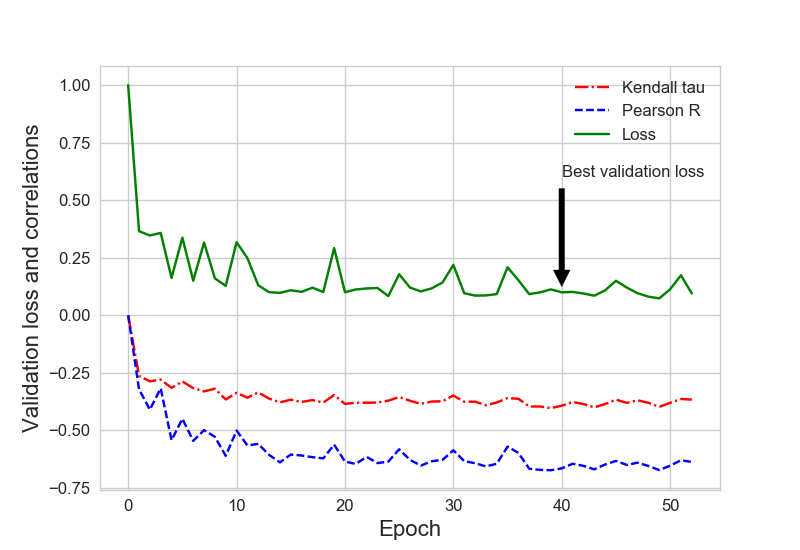
\includegraphics[width=\linewidth]{Fig/kendall_validation.eps}
%
    \caption{Loss, Kendall $\tau$, and Pearson $R$ coefficients
      evaluated on the validation subset during the training
      procedure.  One epoch corresponds to a cycle over all targets in
      the training subset. Models are saved every 10 epochs and the
      arrow shows the minimum validation loss for which a model was
      saved (at epoch 40).}
%
    \label{Fig:TrainingLoss}
\end{figure}

\begin{table}[H]
\begin{center}
\begin{tabular}{ c | c | c | c | c }
    Data & Loss & Pearson $R$ & Spearman $\rho$ & Kendall $\tau$ \\
    \hline
    Training subset     &0.146 &0.71 &0.61 &0.45 \\
    Validation subset   &0.135 &0.71 &0.59 &0.44 \\ \hline
\end{tabular}
    \caption {Performance of the model from epoch 40 on the training
      and validation subsets.}
    \label{Tbl:TrainingResults}
\end{center}
\end{table}
